\section{Auswertung}
\label{sec:Auswertung}
\subsection{Vorbereitung}
Für die Auswertung
werden bestimmte Größen benötigt dazu gehören
zu einem das Dispersionsgebiet $\Delta\lambda$
und das Auflösungsvermögen A der Lummer-Gehrcke-Platte
für die unt
erschiedlichen Wellenlängen $\lambda=\SI{643.8}{\nano\meter}$
und $\lambda=\SI{480.0}{\nano\meter}$.
Das Dispersionsgebiet lässt sich durch die Formel(ADD) berechen
und für das Auflösungsvermögen wird die Formel (ADD) verwendet.


Diese sind in der Tabelle  \ref{tab:vorbereitung} aufgelistet.
\begin{table}
  \centering
  \caption{Berechnete Werte für die Landé-Faktoren der Orbitale.}
  \label{tab:vorbereitung}
  \begin{tabular}{c c c}
    \toprule
       \lambda / \si{\nano\meter}  &  \delta\lambda  & A \\
     \midrule
    643,8  &  4,89e-11 &  1,96e-13 \\
    480,0  &  2,70e-11 &  1,08e-13 \\
    \bottomrule
  \end{tabular}
\end{table}




\subsection{Theoretische Werte}
Zu Beginn können mit Hilfe der Formel \eqref{eqn:lande}
die theoretischen Werte der Lande-Faktoren
für die entsprechenden Orbitale ausgerechnet werden.
Die Berechneten Werte sind in der Tabelle \ref{tab:theo1}
zu finden.

\begin{table}
  \centering
  \caption{Theoretische Werte für die Landé-Faktoren der Orbitale.}
  \label{tab:theo1}
  \begin{tabular}{c c c c c c}
    \toprule
& Orbital  & S   &  L & J  & $g_j$ \\
    \midrule
Rot & $^1P_1$ & 0 & 1 & 1 & 1,0\\
&$^1D_2$& 0 & 2 & 2 & 1,0\\
Blau&$^3S_1$& 1 & 0 & 1 & 2,0\\
&$^3P_1$& 1 & 2 & 1 & 1,5\\
    \bottomrule
  \end{tabular}
\end{table}

Deweiteren könnnen die Lané-Faktoren für Übergänge
bei dem anormalen Zeeman-Effekt berechnet werden. Dafür werden nur
Übergänge zwischen Orbitale, die einen Spin $S\neq0$, besitzen betrachtet (Blaues Licht).
Die Berechneten Werte sind in der Tabelle \ref{tab:theo2}
zu finden.

\begin{table}
  \centering
  \caption{Theoretische Werte für die Landé-Faktoren $g_{ji}$ für Übergänge bei
  dem der annormale Zeeman-Effekt berücksichtigt werden muss.}
  \label{tab:theo2}
\begin{tabular}{c c c c c c c}
  \toprule
Rot      &            &  \multicolumn{2}{c}{$^1P_1$}  & \multicolumn{2}{c}{$^1D_2$} &    \\
      & $\Delta m$ &   $m_1$&  $m_1g_1$            & $m_2$    & $m_2g_2$         & $g_{ij}$\\
\midrule
$\sigma$ &  -1   &    1 &  1,0     &  0  & 0,0  &  1,0  \\
       &       &    0 &  0,0     & -1  & -1,0  &  1,0  \\
$\pi$    &   0   &    1 &  1,0     &  1  &  1,0  &  0,0  \\
       &       &    0 &  0,0     &  0  & 0,0  &  0,0  \\
       &       &   -1 & -1,0     & -1  & -1,0 &  0,0 \\
$\sigma$ &  +1   &    0 &  0,0     &  1  & 1,0  & -1,0  \\
       &       &   -1 & -1,0     &  0  & 0,0  & -1,0  \\
\midrule
\midrule
Blau &            &  \multicolumn{2}{c}{$^3P_1$}  & \multicolumn{2}{c}{$^3P_1$} &    \\
& $\Delta m$ &   $m_1$&  $m_1g_1$            & $m_2$    & $m_2g_2$         & $g_{ij}$\\
  \midrule
$\sigma$ &  -1   &    1 &  2,0     &  0  & 0,0  &  2,0  \\
       &       &    0 &  0,0     & -1  & 1,5  &  1,5  \\
$\pi $   &   0   &    1 &  2,0     &  1  & 1,5  &  0,5  \\
       &       &    0 &  0,0     &  0  & 0,0  &  0,0  \\
       &       &   -1 & -2,0     & -1  & -1,5 & -0,5  \\
$\sigma$ &  +1   &    0 &  0,0     &  1  & 1,5  & -1,5  \\
       &       &   -1 & -2,0     &  0  & 0,0  & -2,0  \\
\bottomrule
\end{tabular}
\end{table}

\subsection{Hysterese}
Es wurde eine Hysteresekurve für den verwendeten Elektromagneten aufgenommen.
Die Tabelle \ref{tab:hyst} enthält die Messwerte von des Magnetfeld $B$
in Abhängigkeit von dem  Strom $I$. Diese sind wiederum
in der Abblidung \ref{fig:hyst} aufgetragen.
\begin{table}
  \centering
  \caption{Messwerte für die Hysterese}
  \label{tab:hyst}
\begin{tabular}{c c | c c}
  \toprule
 Strom $I/\si{\ampere}$  & Magnetfeld $B/\si{\milli\tesla}$  & $I/\si{\ampere}$ & $B/\si{\milli\tesla}$ \\
  \midrule
  1   &  70  &  20  &  1015 \\
  2   &  120 &  19  &   986 \\
  3   &  177 &  18  &   960 \\
  4   &  239 &  17  &   931 \\
  5   &  297 &  16  &   897 \\
  6   &  348 &  15  &   859 \\
  7   &  420 &  14  &   807 \\
  8   &  468 &  13  &   744 \\
  9   &  528 &  12  &   687 \\
  10  &  584 &  11  &   611 \\
  11  &  649 &  10  &   544 \\
  12  &  714 &   9  &   498 \\
  13  &  759 &  8   &   447 \\
  14  &  799 &  7   &   377 \\
  15  &  837 &  6   &   322 \\
  16  &  894 &  5   &   275 \\
  17  &  923 &  4   &   207 \\
  18  &  965 &  3   &   131 \\
  19  &  984 &  2   &   104 \\
  20  &  1015 &  1   &    50 \\
  \bottomrule
\end{tabular}
\end{table}


\begin{figure}
   \centering
   \includegraphics[width=0.7\textwidth]{build/plot_hyst.pdf}
   \caption{Hysteresekurve des verwendeten Elektromagneten.}
   \label{fig:hyst}
 \end{figure}

Um Später die Benötigten B-Felder Zu bestimmen wird eine Ausgleichsrechnung
an den Messwerten bei steigendem Strom durch geführt.
Als Ansatz wird die Funktion
\begin{align}
B(I)=A \cdot \arctan(\frac{I-I_0}{C}) \label{eqn:hyst}
\end{align}
verwendet.
Es ergeben sich für die Parameter die folgenden Werte:
\begin{align}
  A=\SI{1.39(7)e3}{\milli\tesla}&   &I_0=\SI{0.21(13)}{\ampere}&  &C=\SI{21.6(16)}{\ampere}.
\end{align}

\subsection{Gemessene Landé-Faktoren}
Um aus den Messergebnissen den
Landé-Faktoren zu berechnen, müssen zunächst aus den
aufgenommenen Bildern \ref{fig:rot}-\ref{fig:blau_pi} $\Delta s$ und $\delta s$ bestimmt werden.
\footnote{$\Delta s$ und $\delta s$ wurden mit Hilfe des Lineartools von Paint gemessen.}
Die entsprechen Werte sind in der Tabelle \ref{tab:ds}
aufgelistet.
\subsubsection{\texorpdfstring{$\sigma$}{TEXT}-Rot}
\begin{figure}
   \centering
   \begin{subfigure}{0.9\textwidth}
     \centering
     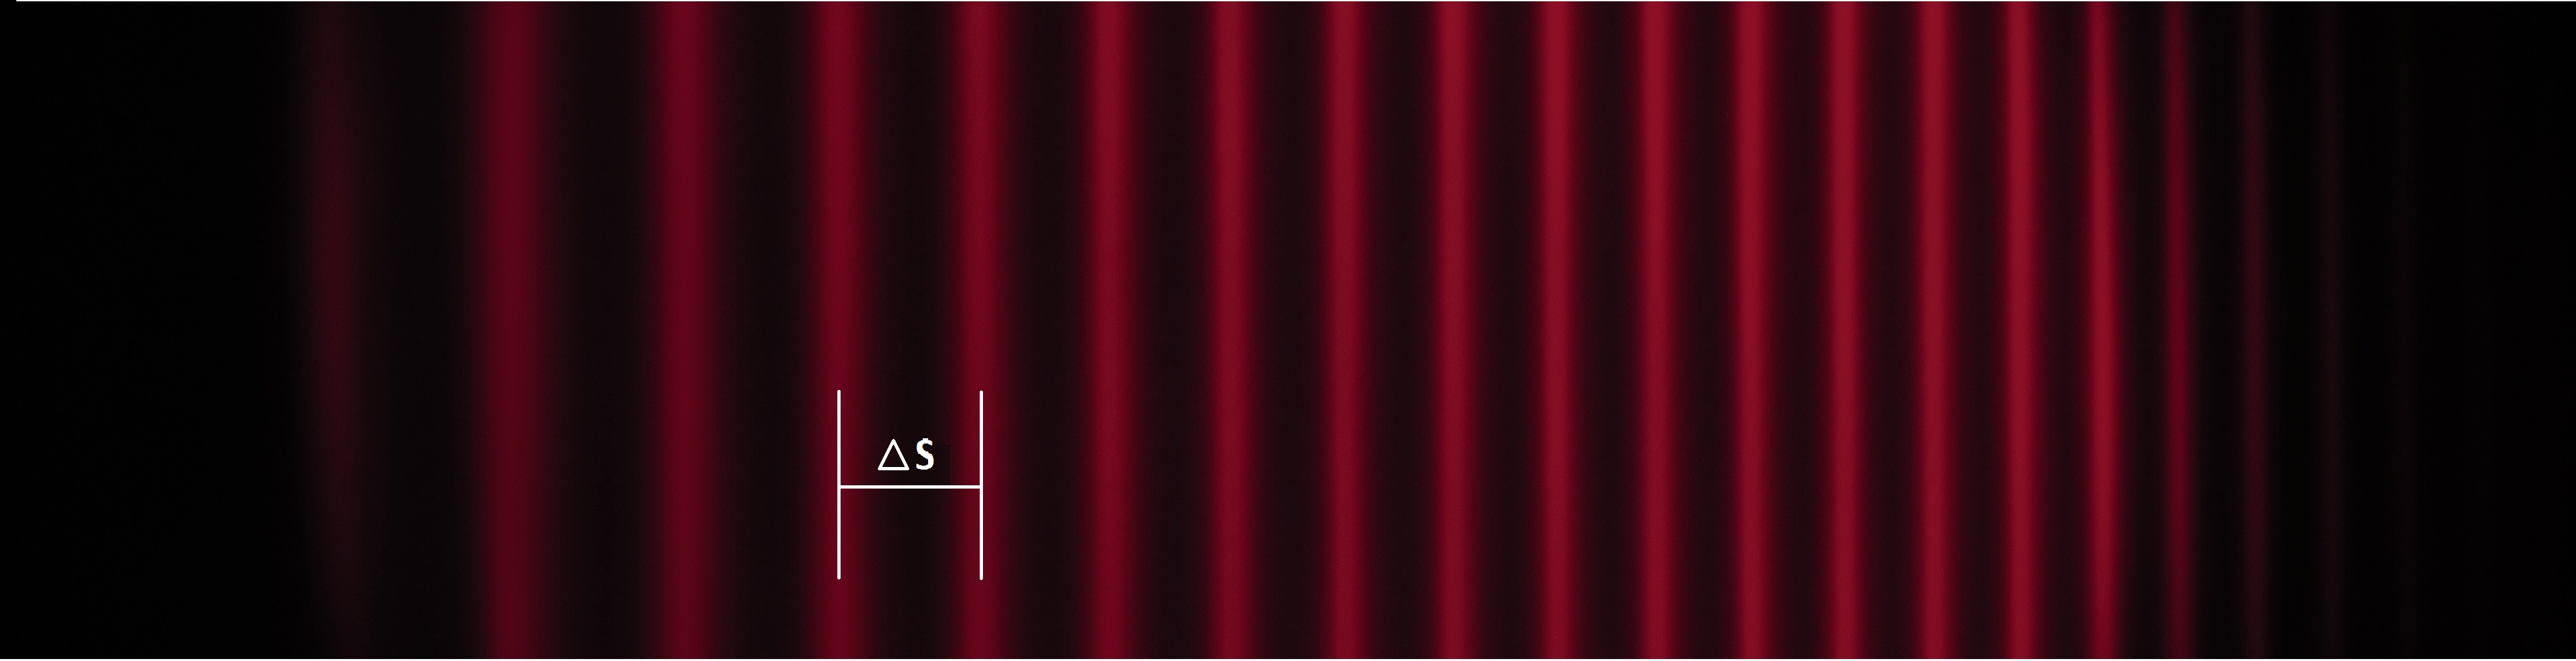
\includegraphics[width=1\textwidth]{rot_sigma_B=0.jpg}
     \caption{}
     \label{fig:rotB=0}
   \end{subfigure}
   \begin{subfigure}{0.9\textwidth}
     \centering
     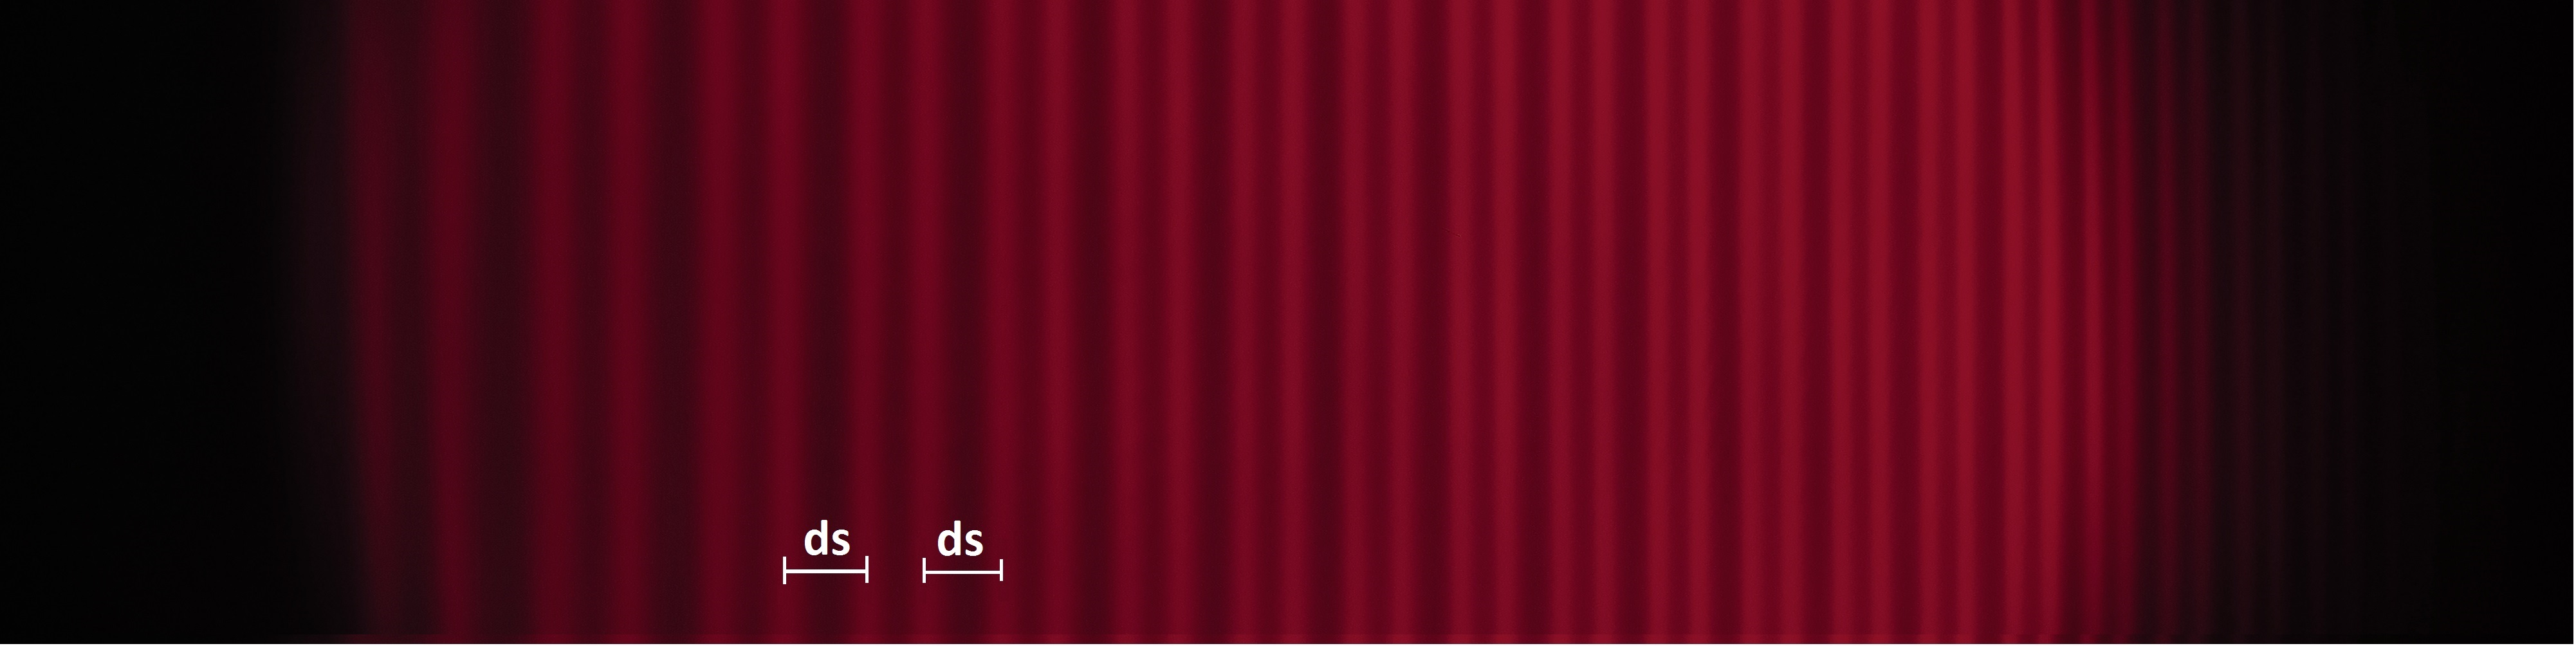
\includegraphics[width=1\textwidth]{rot_sigma_B=!0.jpg}
     \caption{}
     \label{fig:rotB=!0}
   \end{subfigure}
\caption{Interferenzbilder einmal für $B=0$ \ref{fig:rotB=0} und für $B\neq0$ \ref{fig:rotB=!0}}
\label{fig:rot}
\end{figure}
\FloatBarrier
\subsubsection{\texorpdfstring{$\sigma$}{TEXT}-Blau}

\begin{figure}
   \centering
   \begin{subfigure}{0.9\textwidth}
     \centering
     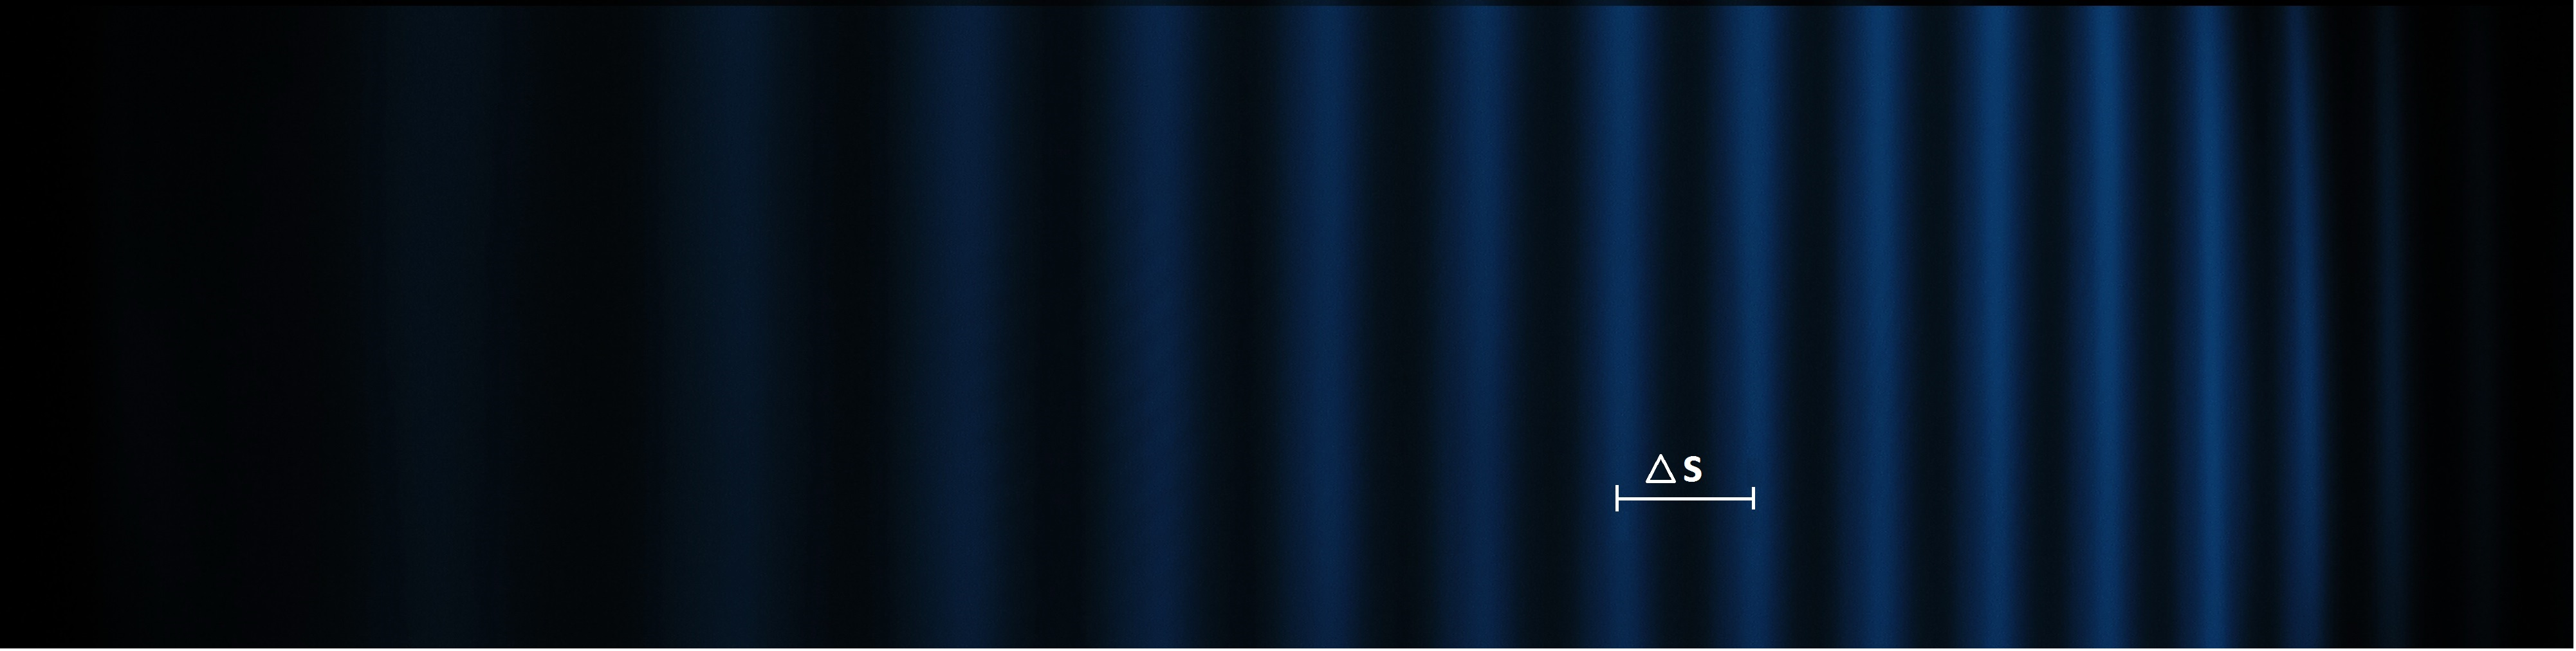
\includegraphics[width=1\textwidth]{blau_sigma_B=0.jpg}
     \caption{}
     \label{fig:blau_sigB=0}
   \end{subfigure}
   \begin{subfigure}{0.9\textwidth}
     \centering
     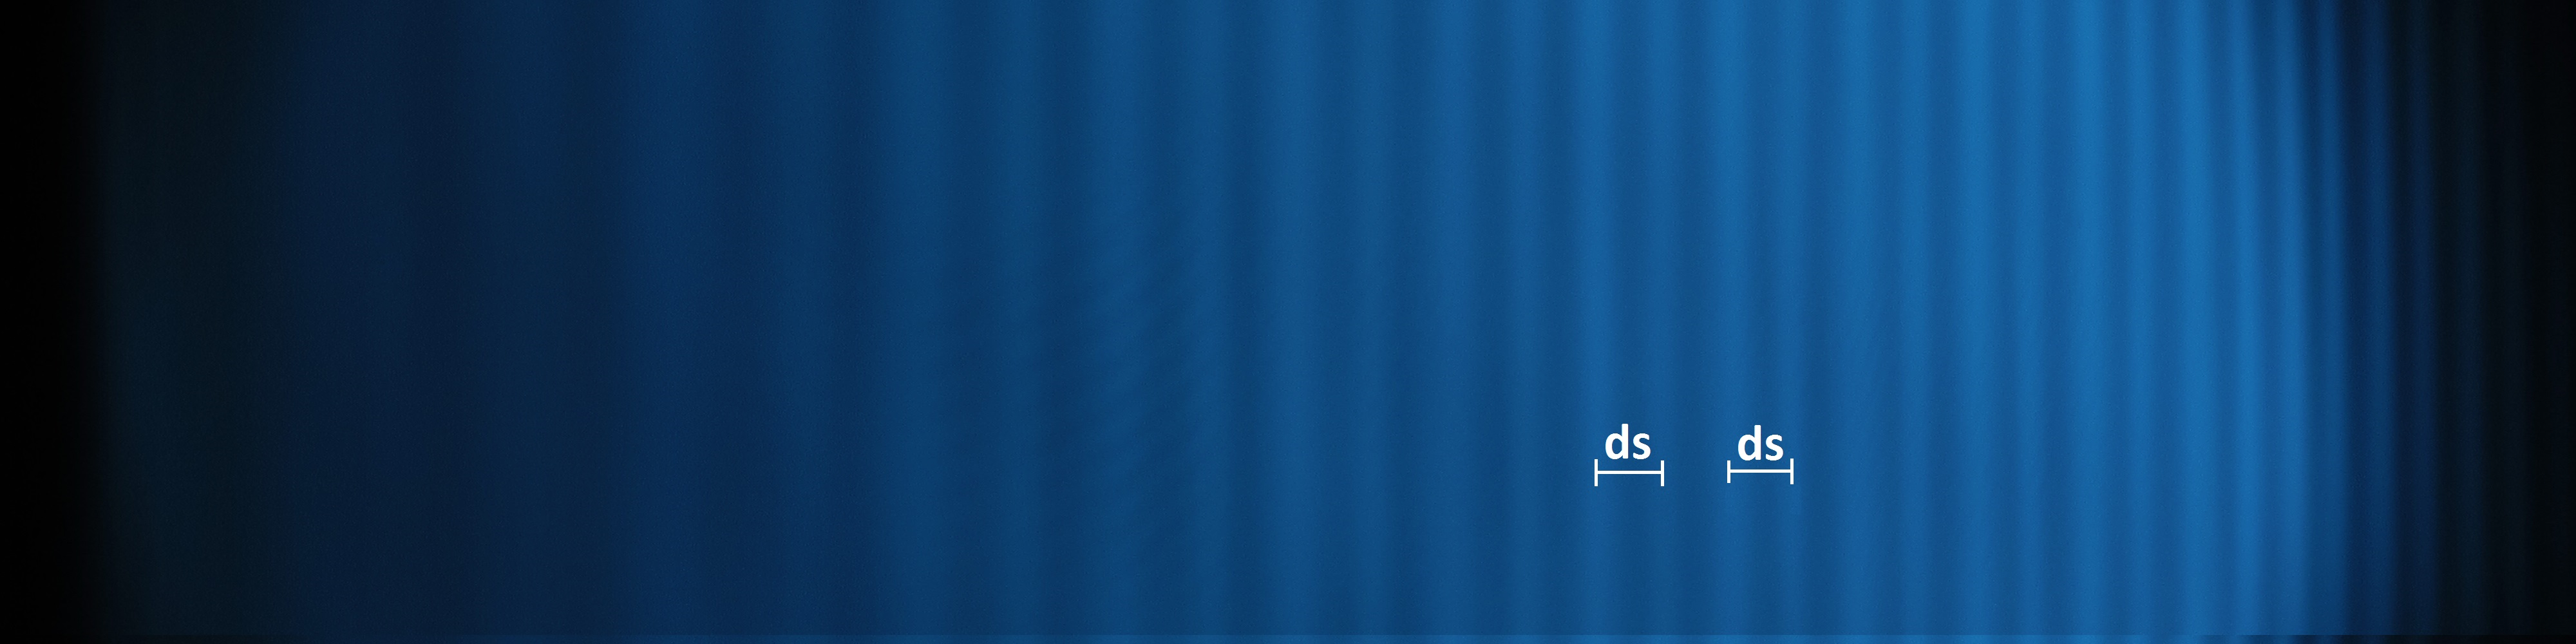
\includegraphics[width=1\textwidth]{blau_sigma_B=!0.jpg}
     \caption{}
     \label{fig:blau_sigB=!0}
   \end{subfigure}
\caption{Interferenzbilder einmal für $B=0$ \ref{fig:blau_sigB=0} und für $B\neq0$ \ref{fig:blau_sigB=!0}}
\label{fig:blau_sig}
\end{figure}



\FloatBarrier
\subsubsection{\texorpdfstring{$\pi$}{TEXT}-Blau}

\begin{figure}
   \centering
   \begin{subfigure}{0.9\textwidth}
     \centering
     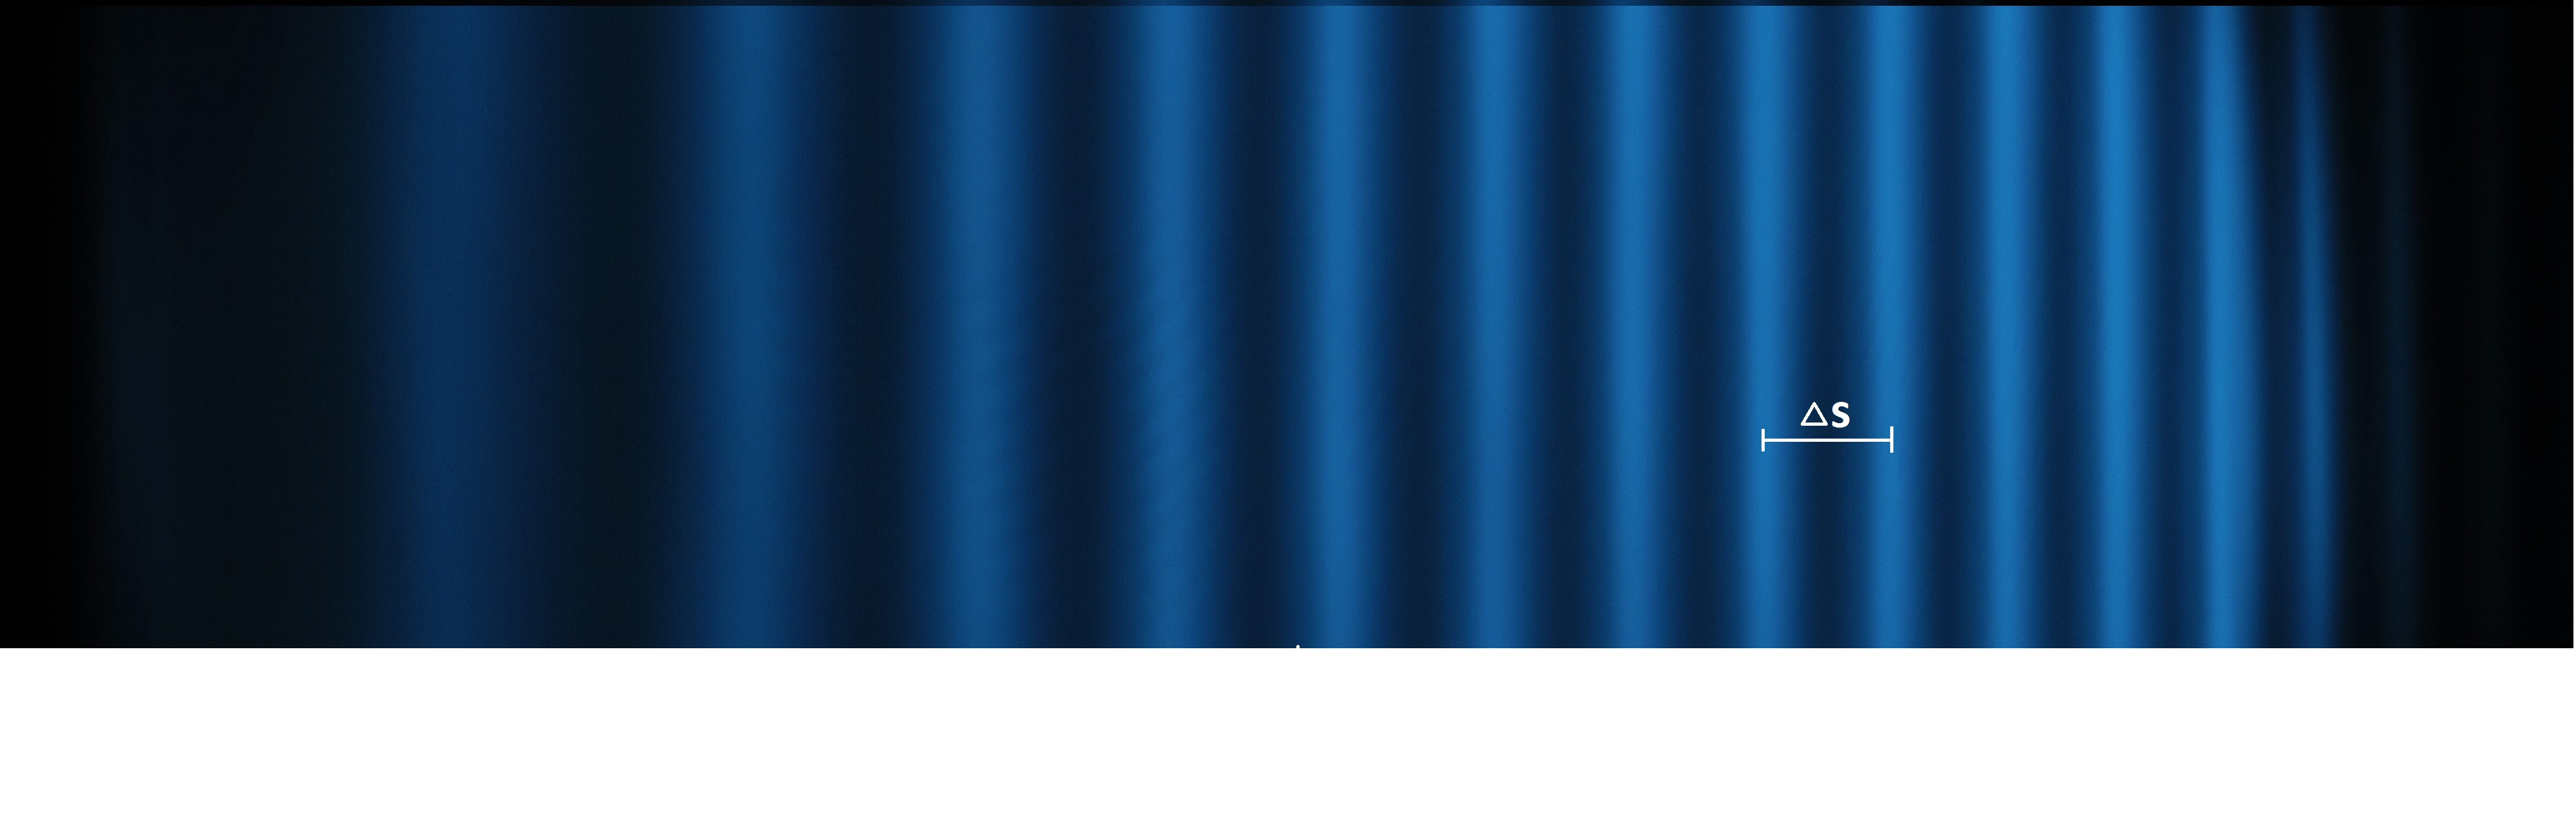
\includegraphics[width=1\textwidth]{blau_pi_B=0.jpg}
     \caption{}
     \label{fig:blau_piB=0}
   \end{subfigure}
   \begin{subfigure}{0.9\textwidth}
     \centering
     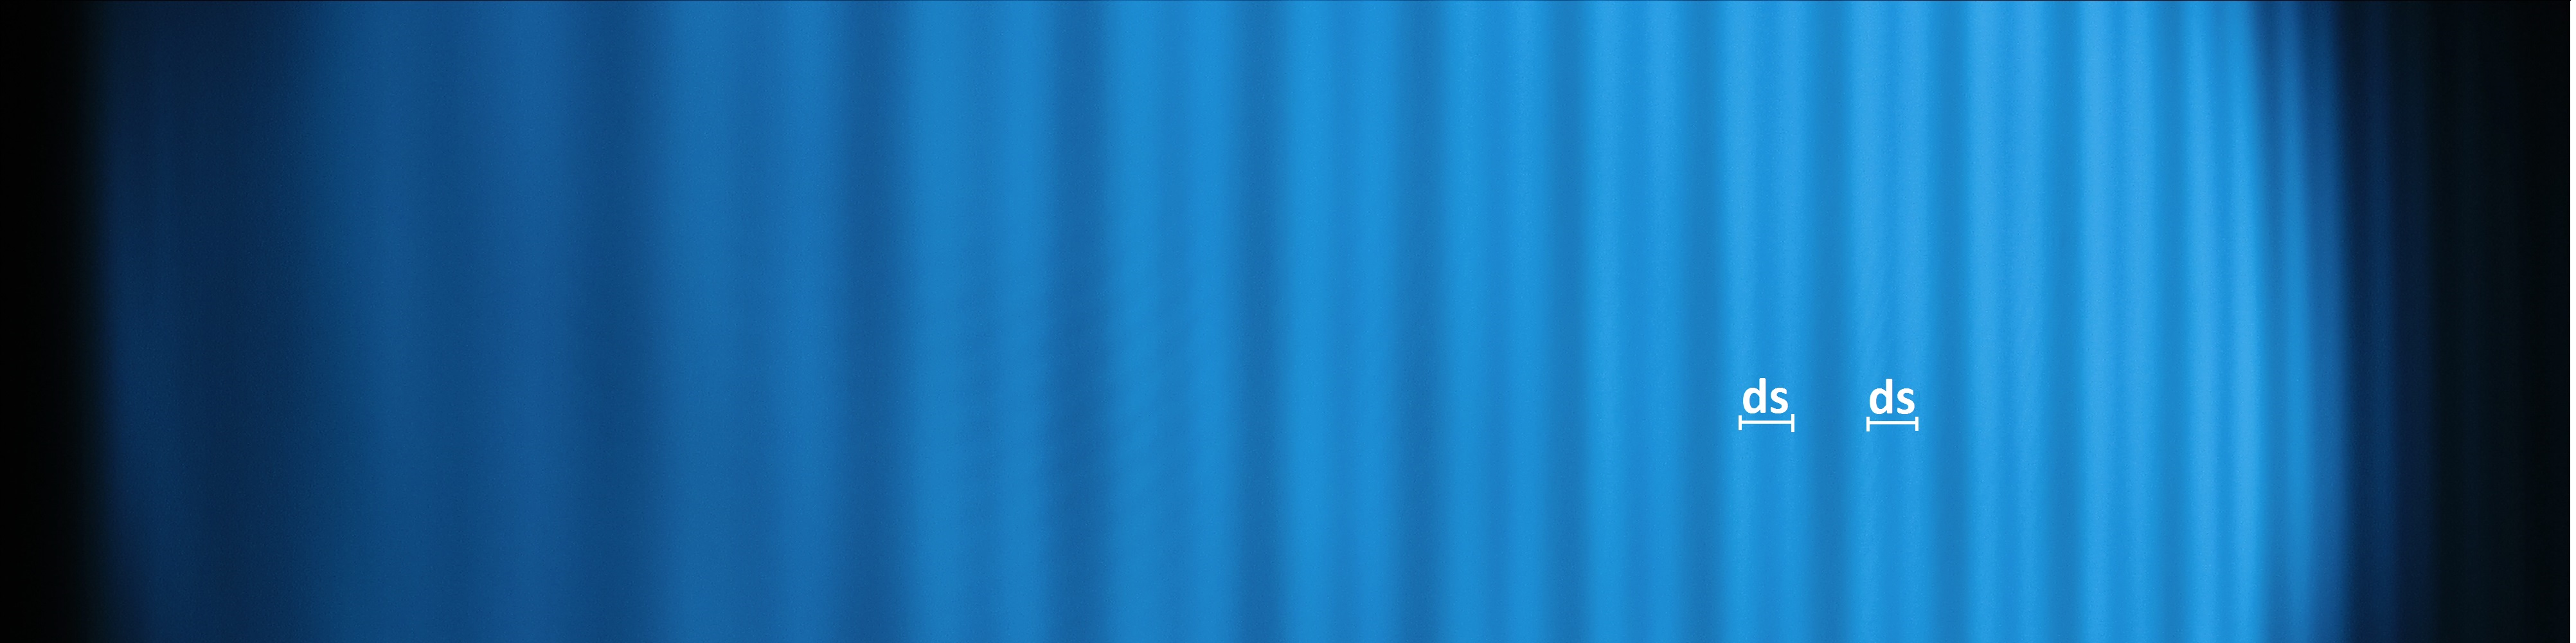
\includegraphics[width=1\textwidth]{blau_pi_B=!0.jpg}
     \caption{}
     \label{fig:blau_piB=!0}
   \end{subfigure}
\caption{Interferenzbilder einmal für $B=0$ \ref{fig:blau_piB=0} und für $B\neq0$ \ref{fig:blau_piB=!0}}
\label{fig:blau_pi}
\end{figure}

\begin{table}
  \centering
  \caption{Messwerte für die $\Delta s$ und $\delta s$}
  \label{tab:ds}
\begin{tabular}{c c c c c c}
  \toprule
&      &  $\Delta s$ & \multicolumn{2}{c}{$\delta s$}& $\overline{\delta s}$ \\
\midrule
Rot&$\sigma$  &   230   &    140 & 115 &128\pm12 \\
\midrule
\midrule
Blau&  $\sigma$ & 210 & 100 & 95 & 97.5\pm2.5 \\
&  $\pi$   & 205 &  80 & 80 &  80\pm0    \\
\bottomrule
\end{tabular}
\end{table}

Aus den gemessenen $\Delta s$ und $\delta s$
für die verschieden Messungen kann durch
die Formel \eqref{eqn:dlam} die
die Wellenlängenänderung
\begin{align}
  \delta\lambda=\frac{\delta s}{\Delta s}\cdot \Delta \lambda_\mathrm{D} \label{eqn:dlam}
\end{align}
bestimmt werden.
Diese kann dafür genutzt werden den
Landé-Faktor $g_{ij}$ über die Formel \eqref{eqn:g_ji} zu berechnen.
\begin{align}
\lvert g_{ij}\rvert=\lvert \frac{\Delta E}{\mu_\mathrm{B}B}\rvert
\intertext{dafür kann $\Delta E$ durch $\delta \lambda$ ausgedrückt werden,
wobei beachtet werden muss, dass $\Delta E$ nicht linear mit $\lambda$ folglich gilt:}
\lvert \Delta E\rvert =\lvert\frac{\partial E}{\partial \lambda} \delta \lambda \rvert= \lvert\frac{hc}{\lambda^2}\delta\lambda\rvert
\intertext{und}
g_{ij}=\frac{hc}{\lambda^2 \mu_\mathrm{B}B} \delta \lambda
\end{align}
In der Tabelle \ref{tab:messgij} sind die berechneten Werte für $\delta \lambda$, $\Delta E$ und $g_{ij}$ aufgelistet
sowie der gemessene Strom $I$ und die Flussdichte $B$, die aus der bestimmten Fit-Funktion \eqref{eqn:hyst} berechnet wird.


\begin{table}
  \centering
  \caption{Messwerte für die $\Delta s$ und $\delta s$}
  \label{tab:messgij}
\begin{tabular}{c c c c c c c}
  \toprule
& & $I/\si{\ampere}$  & $B/\si{\milli\tesla}$ & $\delta\lambda$ /\si{\pico\meter}  &  $\Delta E / \si{\micro\electronvolt}$ & $g_ij$ \\
\midrule
Rot&$\sigma $ & 11,8\pm0,5 & 13,6\pm1,3 & 1,02\pm0,14  \\
\midrule
\midrule
Blau&$\sigma$ &  5,1\pm0,5 & 6,3\pm0,2  &33,7\pm0,9 & 1,88\pm0,26    \\
&  $\pi$      & 17,0\pm0,5 & 5,3\pm0    &28,3\pm0   &  1,53\pm0,04  \\
\bottomrule
\end{tabular}
\end{table}
